% Digital Logic Report Template
% Created: 2020-01-10, John Miller

%==========================================================
%=========== Document Setup  ==============================

% Formatting defined by class file
\documentclass[11pt]{article}

% ---- Document formatting ----
\usepackage[margin=1in]{geometry}	% Narrower margins
\usepackage{booktabs}				% Nice formatting of tables
\usepackage{graphicx}				% Ability to include graphics
\usepackage[section]{placeins}  % Stops floats from happening
\usepackage[labelformat=empty]{caption} % removes figure from captions

%\setlength\parindent{0pt}	% Do not indent first line of paragraphs 
\usepackage[parfill]{parskip}		% Line space b/w paragraphs
%	parfill option prevents last line of pgrph from being fully justified

% Parskip package adds too much space around titles, fix with this
\RequirePackage{titlesec}
\titlespacing\section{0pt}{8pt plus 4pt minus 2pt}{3pt plus 2pt minus 2pt}
\titlespacing\subsection{0pt}{4pt plus 4pt minus 2pt}{-2pt plus 2pt minus 2pt}
\titlespacing\subsubsection{0pt}{2pt plus 4pt minus 2pt}{-6pt plus 2pt minus 2pt}

% ---- Hyperlinks ----
\usepackage[colorlinks=true,urlcolor=blue]{hyperref}	% For URL's. Automatically links internal references.

% ---- Code listings ----
\usepackage{listings} 					% Nice code layout and inclusion
\usepackage[usenames,dvipsnames]{xcolor}	% Colors (needs to be defined before using colors)

% Define custom colors for listings
\definecolor{listinggray}{gray}{0.98}		% Listings background color
\definecolor{rulegray}{gray}{0.7}			% Listings rule/frame color

% Style for Verilog
\lstdefinestyle{Verilog}{
	language=Verilog,					% Verilog
	backgroundcolor=\color{listinggray},	% light gray background
	rulecolor=\color{blue}, 			% blue frame lines
	frame=tb,							% lines above & below
	linewidth=\columnwidth, 			% set line width
	basicstyle=\small\ttfamily,	% basic font style that is used for the code	
	breaklines=true, 					% allow breaking across columns/pages
	tabsize=3,							% set tab size
	commentstyle=\color{gray},	% comments in italic 
	stringstyle=\upshape,				% strings are printed in normal font
	showspaces=false,					% don't underscore spaces
}

% How to use: \Verilog[listing_options]{file}
\newcommand{\Verilog}[2][]{%
	\lstinputlisting[style=Verilog,#1]{#2}
}




%======================================================
%=========== Body  ====================================
\begin{document}

\title{ELC 2137 Lab 05: Intro to Verilog}
\author{Maddie Vorhies}

\maketitle


\section*{Summary}

In this lab, the goal was to get familiar with Verilog and be able to produce a halfadder, fulladder, and an adder/subtractor within Verilog. For this lab it was very important to keep my files organized and adhere to the given folder structure. To begin, I created an RTL project with Basys3 as my default board. The first circuit that I created was a halfadder. For this circuit, as well as the remaining circuits, the file type is system verilog and the location is the Lab05 folder within the correct repository.  To create the halfadder, I added two sources. The first source was the design source, which is what I used to build the halfadder, and the second source was the simulation source, which is what I used to test the halfadder. I also did this for the remaining circuits. The only difference is that I put each simultion source in a different foulder. A halfadder consists of two inputs a and b, and two outputs c and s. I then assigned c = a AND b and s = a XOR b. Now that the half adder is build, I created a simulation source that told vivado where to plug in wires and what inputs to test out. I went through the same process with the remaining circuits. Overall, my results seemed to be successful as my values matched with the expected values.


\section*{Q\&A}

1. What is one thing that you still don't understand about verilog? \newline
I have trouble figuring out the error messages. When I run a simluation and it produces an error message, it takes me a while to figure out what the error actually is. Some of the errors are easy to fix, once I figure out what the porblem is. Other errors are harder to fix even after I find out what is causing the error. I feel like if I were to have a stronger base in verilog, I would either have fewer error messages or I would have a better understanding on how to fix them. 


\section*{Results}


 \begin{figure}[ht]\centering
 	\caption*{halfadder}
	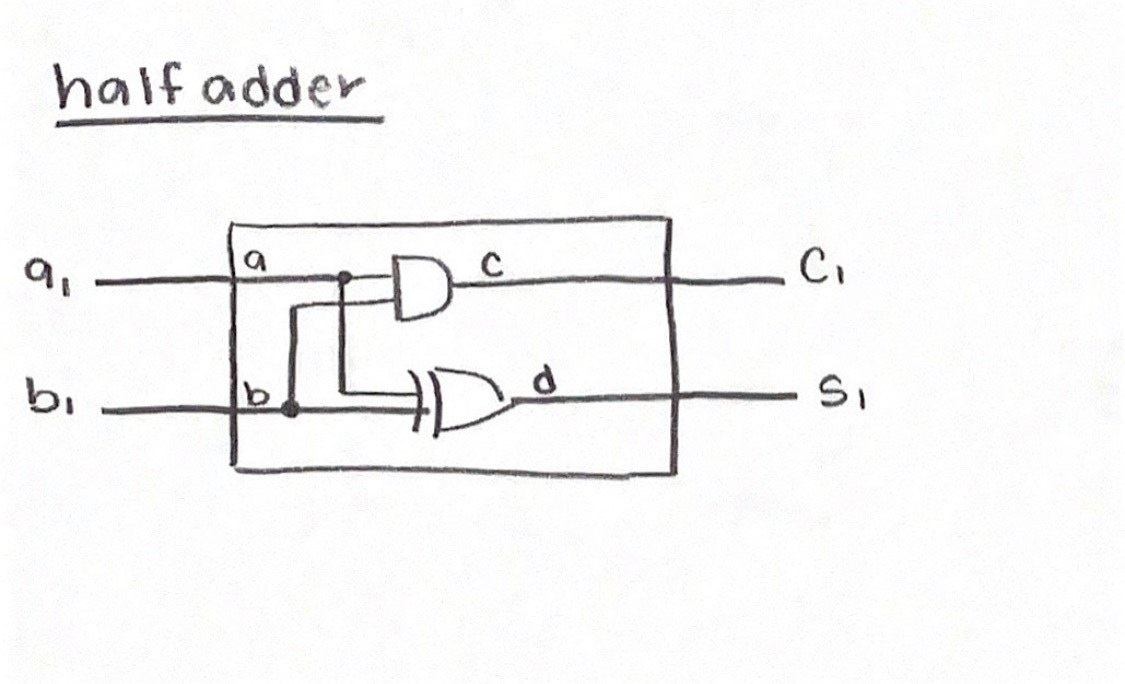
\includegraphics [width=0.3\textwidth,trim=0 0 0 0, clip]{halfadder_blockdiagram}
\end{figure}

\begin{table}[h]\centering
	\begin{tabular}{cc}
		Fulladder & Addsub \\
		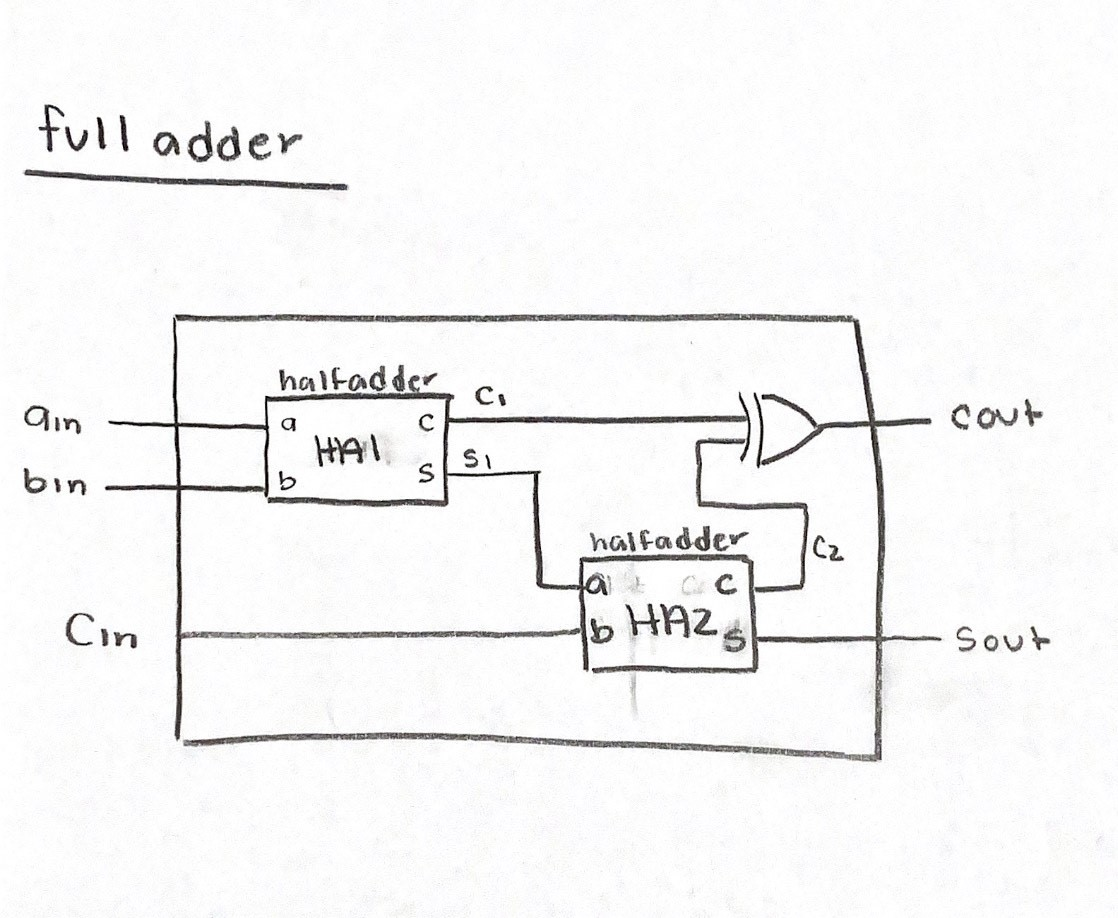
\includegraphics [width=0.4\textwidth,trim=0 0 0 0, clip]{fulladder_blockdiagram} &
		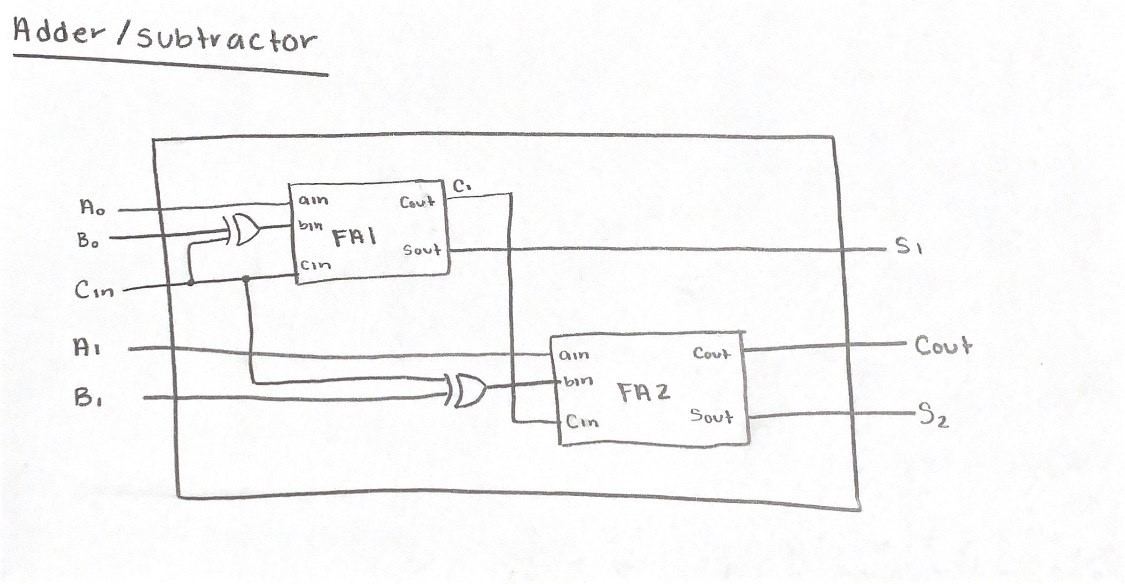
\includegraphics [width=0.55\textwidth,trim=0 0 0 0, clip]{addsub_blockdiagram} \\
	\end{tabular}
	\caption{Block Diagrams}
	\label{fig:sim_with_table}
\end{table}

\begin{figure}[ht]\centering
	\begin{tabular}[ht]{l|cccc}
		Time (ns) & 0 & 10 & 20 & 30 \\
		\midrule
		a & 0 & 1 & 0 & 1\\
		b & 0 & 0 & 1 & 1\\
		\midrule
		c & 0 & 0 & 0 & 1\\
		s & 0 & 1 & 1 & 0\\
		\bottomrule
	\end{tabular}\medskip
	
	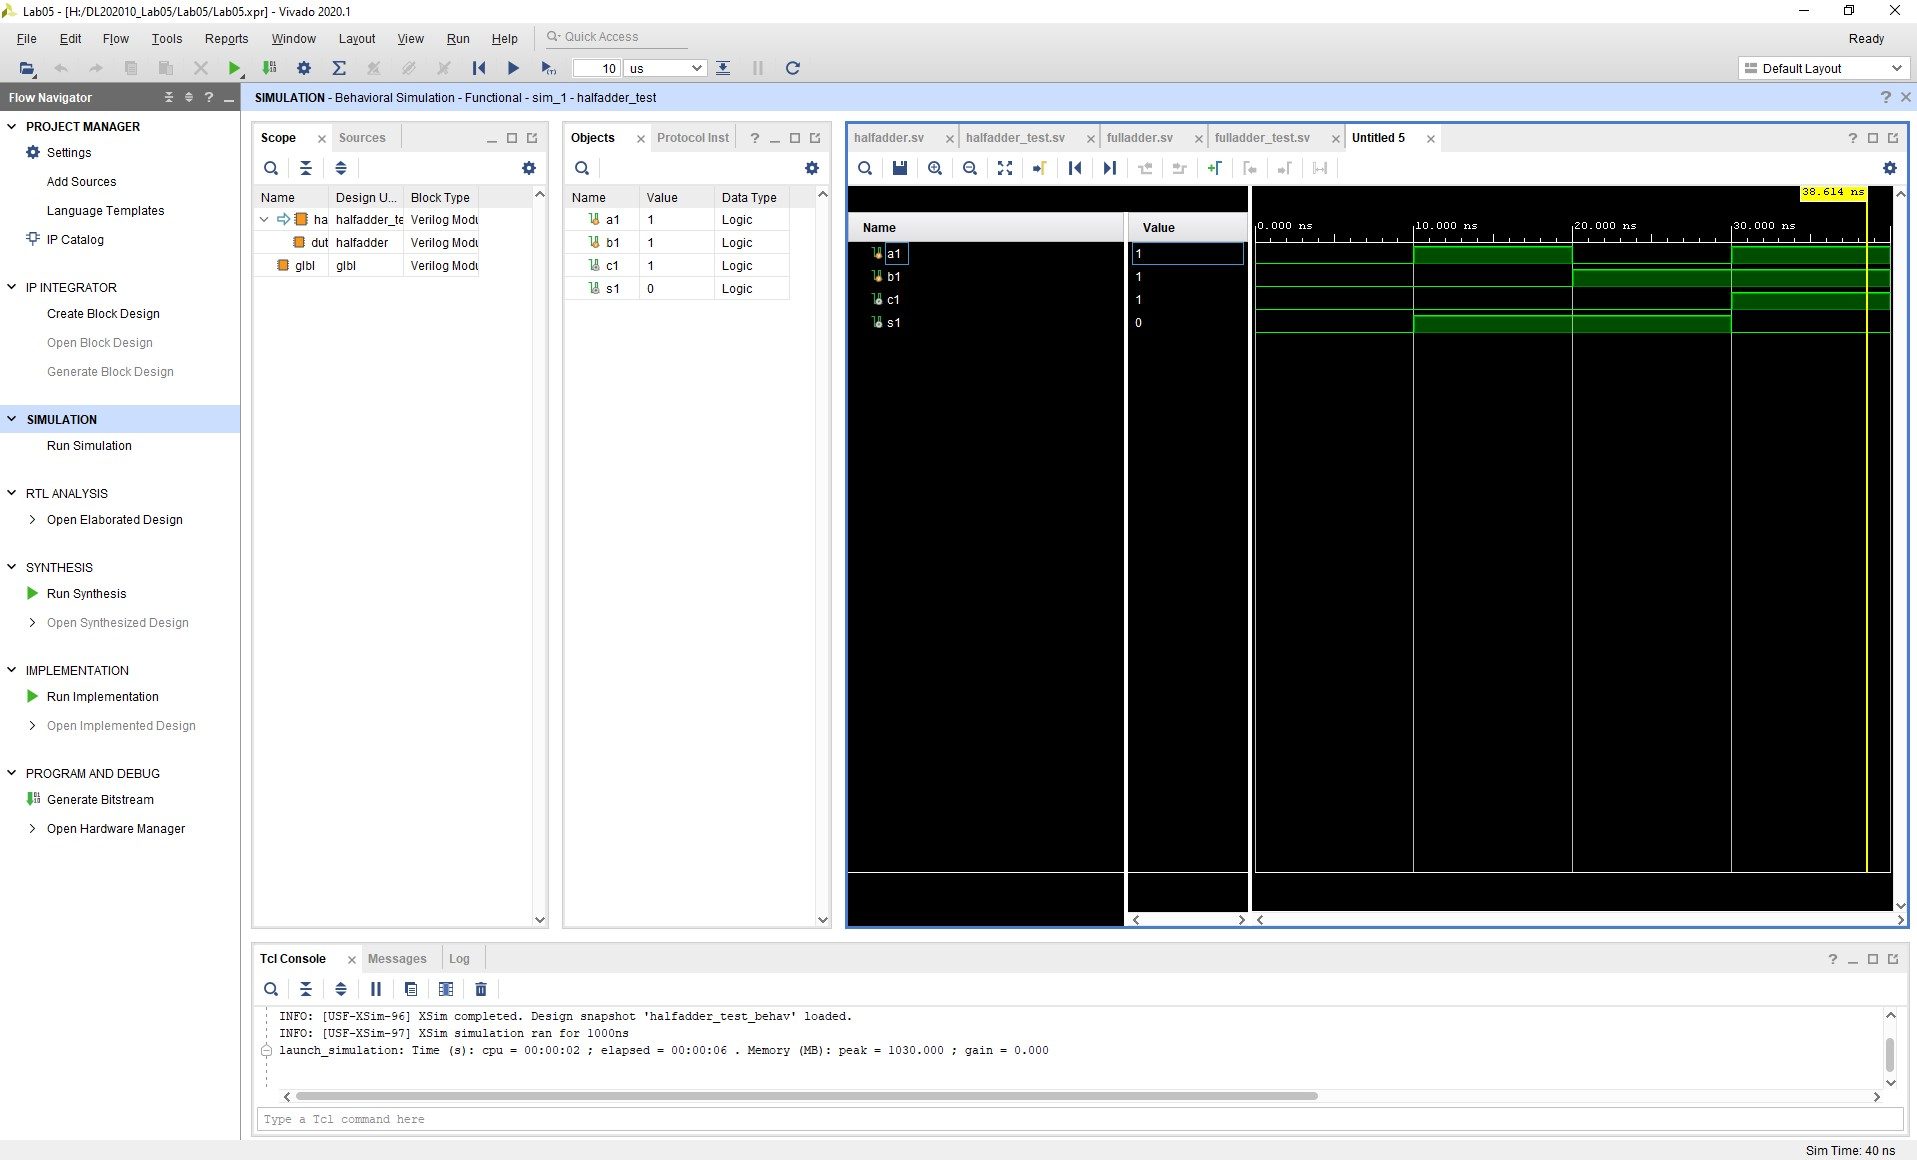
\includegraphics [width=1.0\textwidth,trim=640 600 10 135, clip]{halfadder_pic}
	\caption{Figure 1: Simulation Waveform and ERT of Halfadder}
	\label{fig:sim_with_table}
	
\end{figure}

\begin{figure}[ht]\centering
	\begin{tabular}[ht]{l|cccccccc}
		Time (ns) & 0 & 10 & 20 & 30 & 40 & 50 & 60 & 70 \\
		\midrule
		a & 0 & 1 & 0 & 1 & 0 & 1 & 0 & 1\\
		b & 0 & 0 & 1 & 1 & 0 & 0 & 1 & 1\\
		cin & 0 & 0 & 0 & 0 & 1 & 1 & 1 & 1\\
		\midrule
		cout & 0 & 0 & 0 & 1 & 0 & 1 & 1 & 1\\
		sout & 0 & 1 & 1 & 0 & 1 & 0 & 0 & 1\\
		\bottomrule
	\end{tabular}\medskip
	
	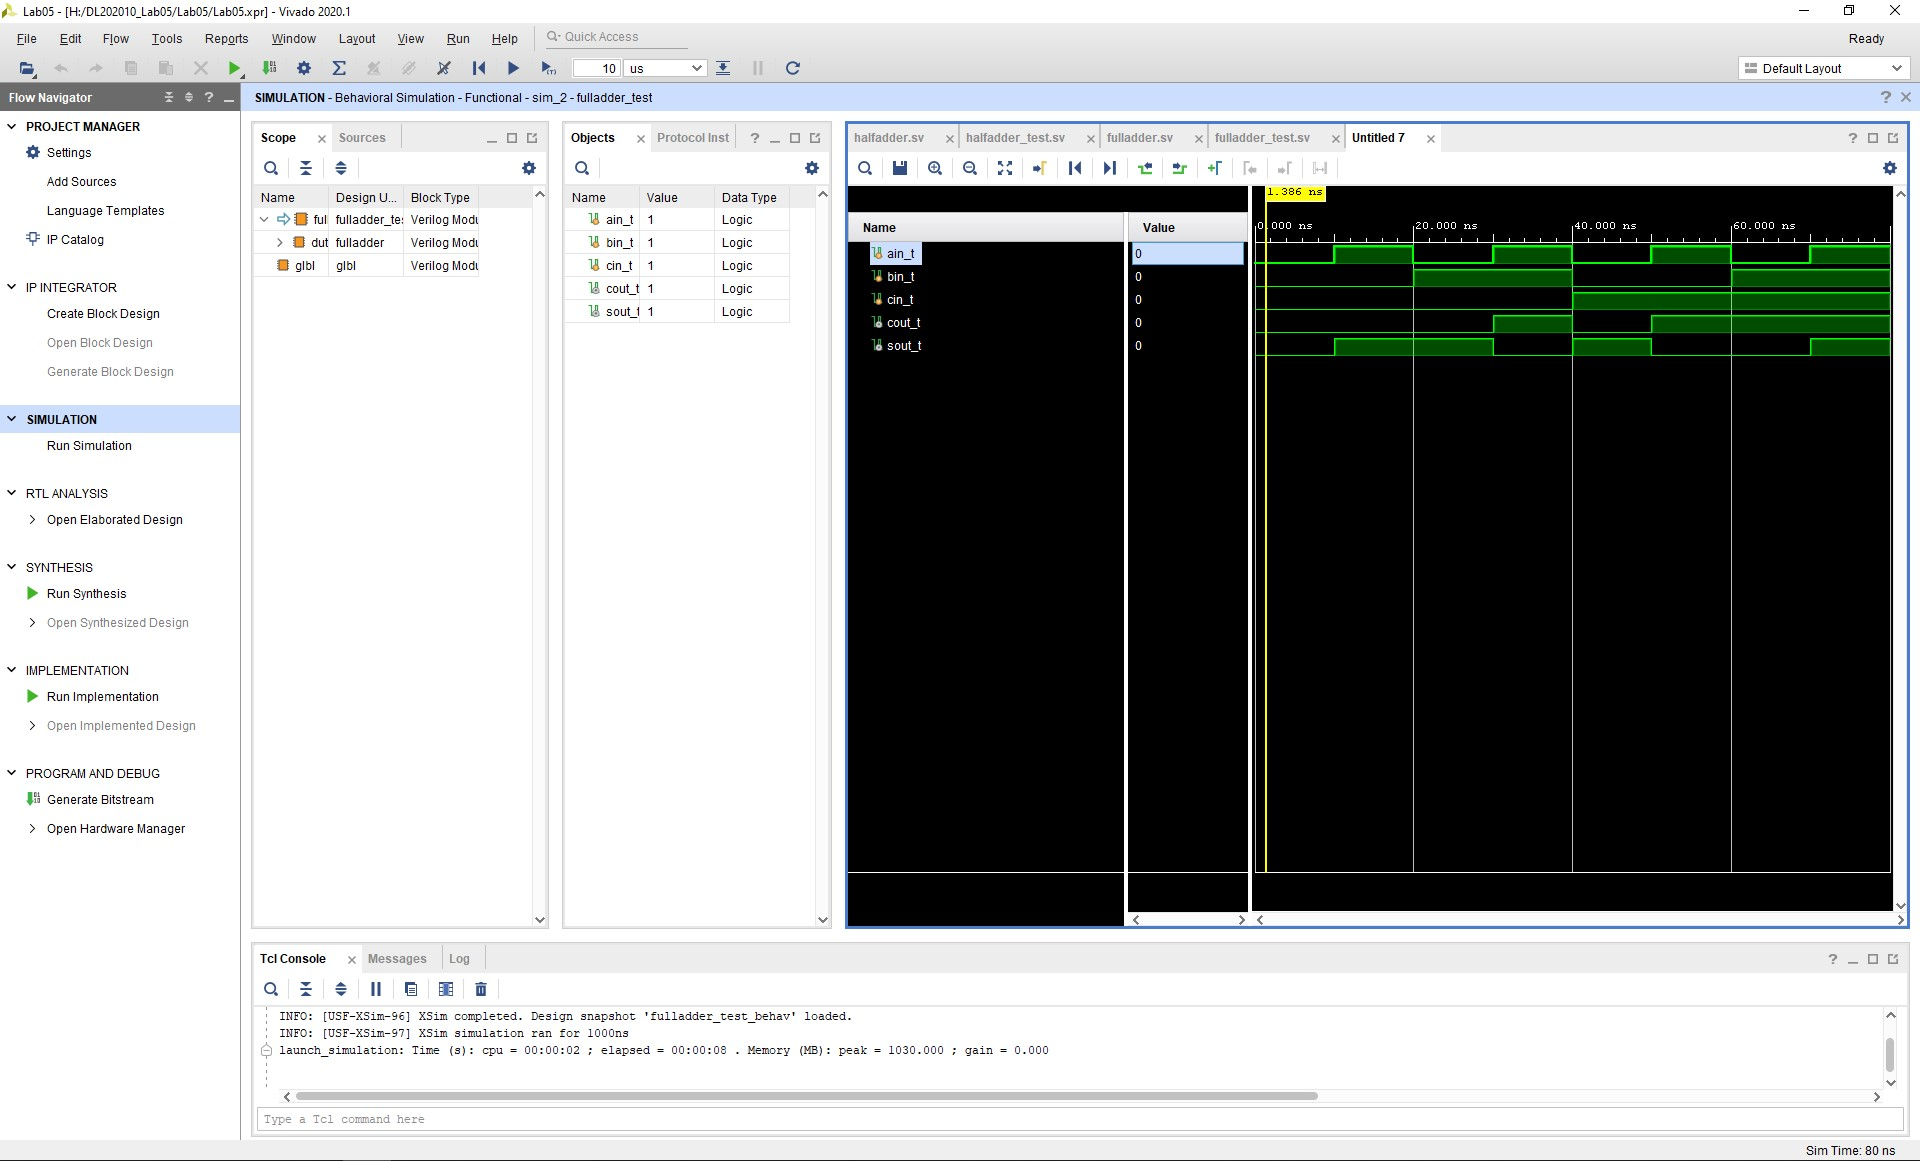
\includegraphics [width=1.0\textwidth,trim=640 600 10 135, clip]{fulladder_pic}
	\caption{Figure 2: Simulation Waveform and ERT of Fulladder}
	\label{fig:sim_with_table}
	
\end{figure}

\begin{figure}[ht]\centering
	\begin{tabular}[ht]{l|cccccccccccc}
		Time (ns) & 0 & 10 & 20 & 30 & 40 & 50 & 60 & 70 & 80 & 90 & 100 & 110\\
		\midrule
		a1 & 0 & 0 & 0 & 0 & 1 & 1 & 0 & 0 & 0 & 0 & 1 & 1\\
		a0 & 0 & 0 & 0 & 1 & 0 & 0 & 0 & 0 & 0 & 1 & 0 & 0\\
		b1 & 0 & 1 & 1 & 0 & 0 & 0 & 0 & 1 & 1 & 0 & 0 & 0\\
		b0 & 1 & 0 & 1 & 1 & 1 & 0 & 1 & 0 & 1 & 1 & 1 & 0\\
		mode & 0 & 0 & 0 & 0 & 0 & 0 & 1 & 1 & 1 & 1 & 1 & 1\\
		\midrule
		s1 & 1 & 0 & 1 & 0 & 1 & 0 & 1 & 0 & 1 & 0 & 1 & 0\\
		s2 & 0 & 1 & 1 & 1 & 1 & 1 & 1 & 1 & 0 & 0 & 0 & 1\\
		cout & 0 & 0 & 0 & 0 & 0 & 0 & 1 & 1 & 1 & 0 & 0 & 0\\
		\bottomrule
	\end{tabular}\medskip
	
	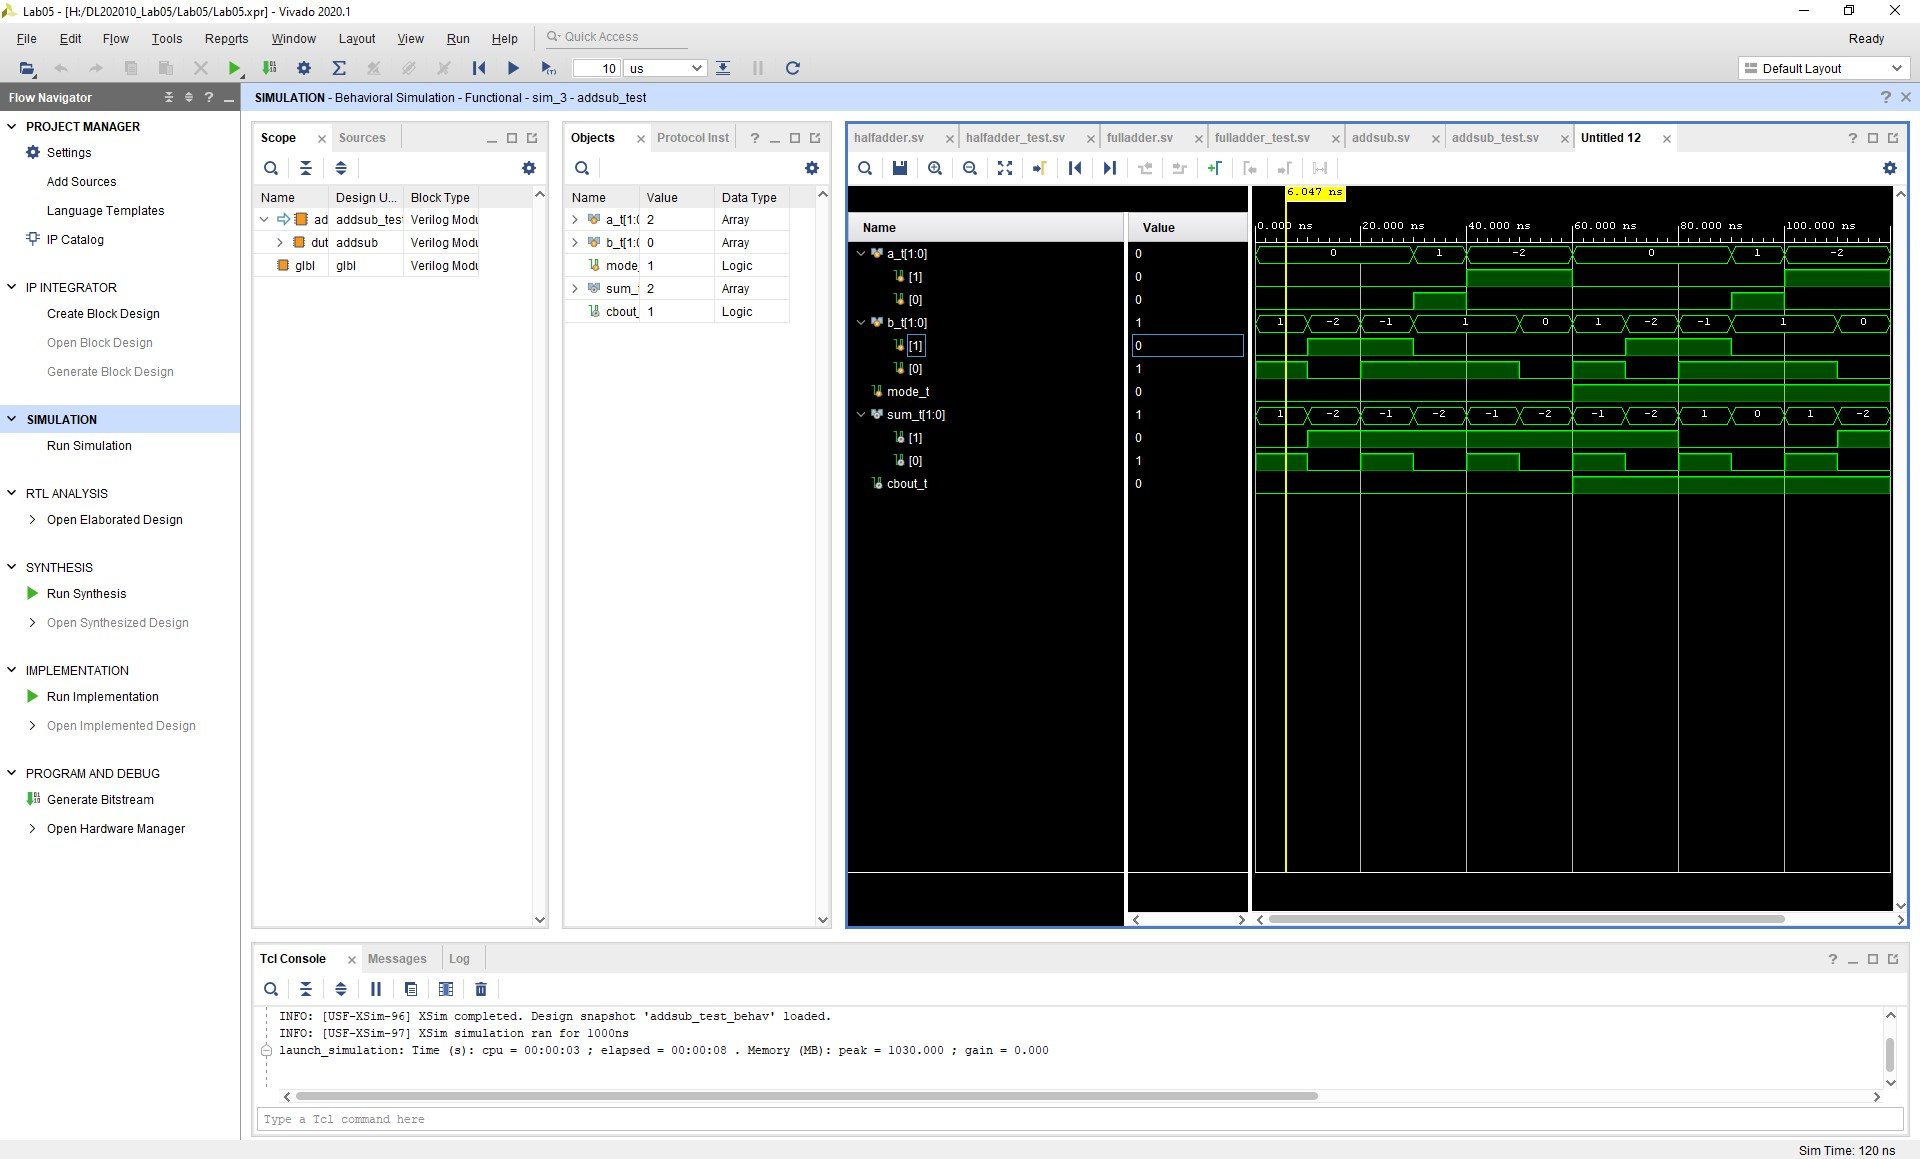
\includegraphics [width=1.0\textwidth,trim=640 450 10 135, clip]{addsub_pic}
	\caption{Figure 3: Simulation Waveform and ERT of AddSub}
	\label{fig:sim_with_table}
	
\end{figure}


\section*{Code}

\begin{lstlisting}

module halfadder(
   input a,
   input b,
   output c,
   output s
   );

   assign c = a & b;
   assign s = a ^ b;

endmodule

\end{lstlisting}

\begin{lstlisting}

module halfadder_test();

   reg a1, b1;
   wire c1, s1;

   halfadder dut (

      .a(a1),
      .b(b1),
      .c(c1),
      .s(s1)
   );

   initial begin 

      a1 = 0; b1 = 0; #10;
      a1 = 1; b1 = 0; #10;
      a1 = 0; b1 = 1; #10;
      a1 = 1; b1 = 1; #10;

      $finish;

   end

endmodule

\end{lstlisting}

\begin{lstlisting}

module fulladder(
   input ain,
   input bin,
   input cin,
   output cout,
   output sout
   );

   wire c1, c2, s1;

   halfadder HA1 (
      .a(ain),
      .b(bin),
      .c(c1),
      .s(s1)
   );

   halfadder HA2 (
      .a(s1),
      .b(cin), 
      .c(c2),
      .s(sout)
   );

   assign cout = c1 ^ c2;

endmodule

\end{lstlisting}

\begin{lstlisting}

module fulladder_test();

   reg ain_t, bin_t, cin_t;
   wire cout_t, sout_t;

   fulladder dut (
      .ain(ain_t),
      .bin(bin_t),
      .cin(cin_t),
      .cout(cout_t),
      .sout(sout_t)
   );

   initial begin 

      cin_t = 0; bin_t = 0; ain_t = 0; #10;
      cin_t = 0; bin_t = 0; ain_t = 1; #10;
      cin_t = 0; bin_t = 1; ain_t = 0; #10;
      cin_t = 0; bin_t = 1; ain_t = 1; #10;
      cin_t = 1; bin_t = 0; ain_t = 0; #10;
      cin_t = 1; bin_t = 0; ain_t = 1; #10;
      cin_t = 1; bin_t = 1; ain_t = 0; #10;
      cin_t = 1; bin_t = 1; ain_t = 1; #10;

      $finish;

   end

endmodule

\end{lstlisting}

\begin{lstlisting}

module addsub(
   input [1:0] a, b,
   input mode,
   output [1:0] sum,
   output cbout
   );

   wire c1, c2;
   wire [1:0] b_n;

   assign b_n[0] = b[0] ^ mode;
   assign b_n[1] = b[1] ^ mode;

   fulladder FA1 (
      .ain(a[0]), .bin(b_n[0]), .cin(mode),
      .cout(c1), .sout(sum[0])
   );

   fulladder FA2 (
      .ain(a[1]), .bin(b_n[1]), .cin(c1),
      .cout(c2), .sout(sum[1])
   );

   assign cbout = c2 ^ mode;


endmodule

\end{lstlisting}

\begin{lstlisting}

module addsub_test();

   reg [1:0] a_t, b_t;
   reg mode_t;
   wire [1:0] sum_t;
   wire cbout_t;

   addsub dut (

      .a(a_t),
      .b(b_t),
      .mode(mode_t),
      .sum(sum_t),
      .cbout(cbout_t)
   );

   initial begin 

      mode_t = 0; a_t[1] = 0; a_t[0] = 0; b_t[1] = 0; b_t[0] = 1; #10;
      mode_t = 0; a_t[1] = 0; a_t[0] = 0; b_t[1] = 1; b_t[0] = 0; #10;
      mode_t = 0; a_t[1] = 0; a_t[0] = 0; b_t[1] = 1; b_t[0] = 1; #10;
      mode_t = 0; a_t[1] = 0; a_t[0] = 1; b_t[1] = 0; b_t[0] = 1; #10;
      mode_t = 0; a_t[1] = 1; a_t[0] = 0; b_t[1] = 0; b_t[0] = 1; #10;
      mode_t = 0; a_t[1] = 1; a_t[0] = 0; b_t[1] = 0; b_t[0] = 0; #10;
      mode_t = 1; a_t[1] = 0; a_t[0] = 0; b_t[1] = 0; b_t[0] = 1; #10;
      mode_t = 1; a_t[1] = 0; a_t[0] = 0; b_t[1] = 1; b_t[0] = 0; #10;
      mode_t = 1; a_t[1] = 0; a_t[0] = 0; b_t[1] = 1; b_t[0] = 1; #10;
      mode_t = 1; a_t[1] = 0; a_t[0] = 1; b_t[1] = 0; b_t[0] = 1; #10;
      mode_t = 1; a_t[1] = 1; a_t[0] = 0; b_t[1] = 0; b_t[0] = 1; #10;
      mode_t = 1; a_t[1] = 1; a_t[0] = 0; b_t[1] = 0; b_t[0] = 0; #10;

      $finish;

   end

endmodule

\end{lstlisting}

\end{document}
